\section{Evaluation and Experiments}

\subsection{Evaluation Framework}

This project adopts a localized RAGAS evaluation framework that does not depend
on OpenAI API, ensuring the privacy and consistency of evaluation.

\subsubsection{Judge Model Configuration}

The system registers the locally deployed Qwen2.5-72B model as RAGAS's
judge\_model, responsible for scoring system answers. If resource constraints
are encountered, it is allowed to downgrade to the Qwen2.5-7B model combined
with manual verification.

\subsubsection{Core Quantitative Metrics}

The RAGAS evaluation framework produces the following core metric scores (0.0 -
1.0) for each answer in the test set:

\begin{enumerate}
    \item \textbf{Context Precision}: Measures whether document chunks that truly contain answer-related information are ranked at the top among the retrieved Top-K document chunks.
    \item \textbf{Faithfulness}: Measures whether the answer finally generated by the large language model is 100% derived from the retrieved document chunks (Context) without fabricating financial data.
    \item \textbf{Answer Relevancy}: Measures whether the answer directly addresses the user's original question.
\end{enumerate}

\subsection{Standardized Test Set}

To ensure horizontal comparability of scores between different phases (Phase 1
vs Phase 2) and different chunking strategies, the system fixed a financial
test question bank containing 20 questions (`data/test\_set.json`).

The test set covers the following four dimensions (5 questions each) to
comprehensively evaluate the system's "fine-grained extraction" and "macro
summarization" capabilities:

\begin{enumerate}
    \item \textbf{Factoid Q\&A}: Tests the system's ability to extract specific data from reports.
    \item \textbf{Reasoning}: Tests the system's ability to analyze causal relationships in reports.
    \item \textbf{Summarization}: Tests the system's ability to macro-summarize report content.
    \item \textbf{Artifact Generation}: Tests the system's ability to generate structured artifacts according to specific formats.
\end{enumerate}

\subsection{Baseline Evaluation}

The system performed baseline index construction and evaluation to establish a
reference point for performance comparison:

\begin{figure}[H]
    \centering
    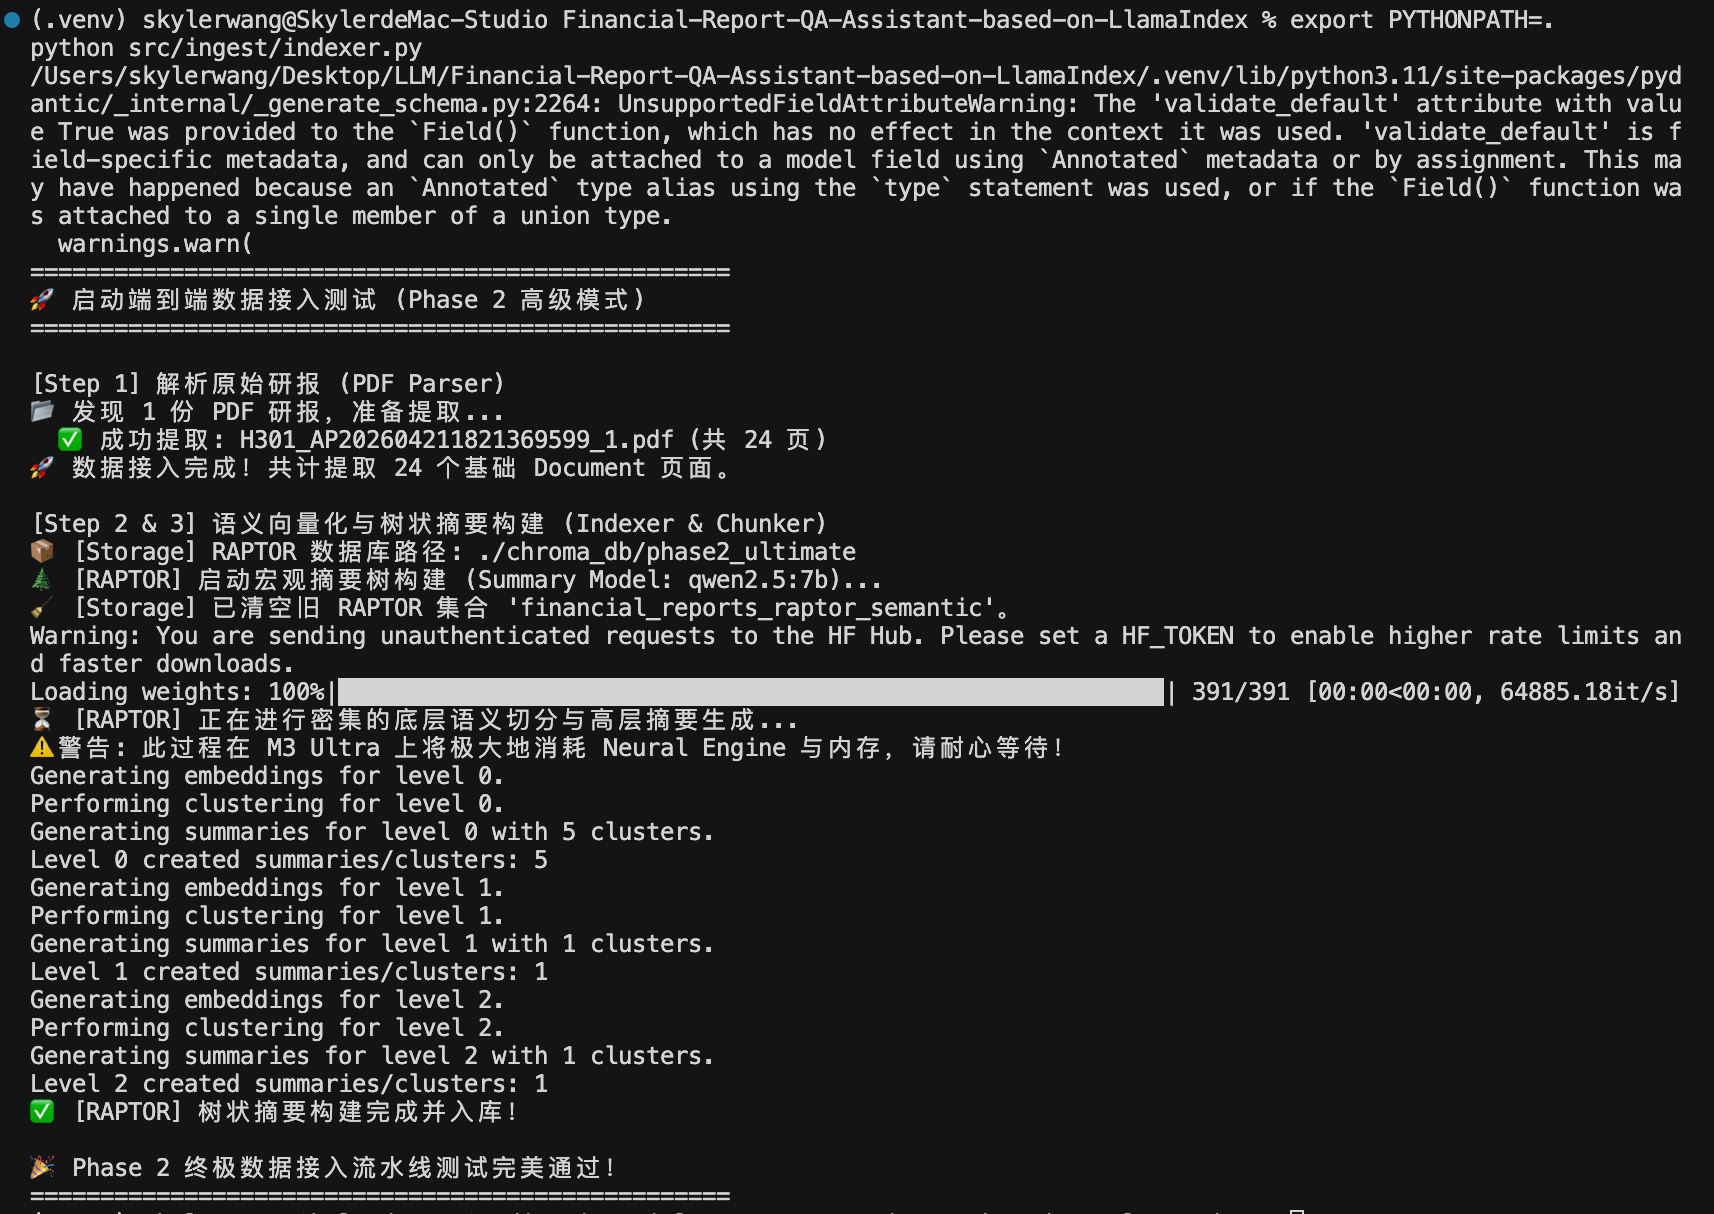
\includegraphics[width=0.8\textwidth]{image/prompts/build.png}
    \caption{Baseline Index Construction}
    \label{fig:baseline_build}
\end{figure}

\begin{figure}[H]
    \centering
    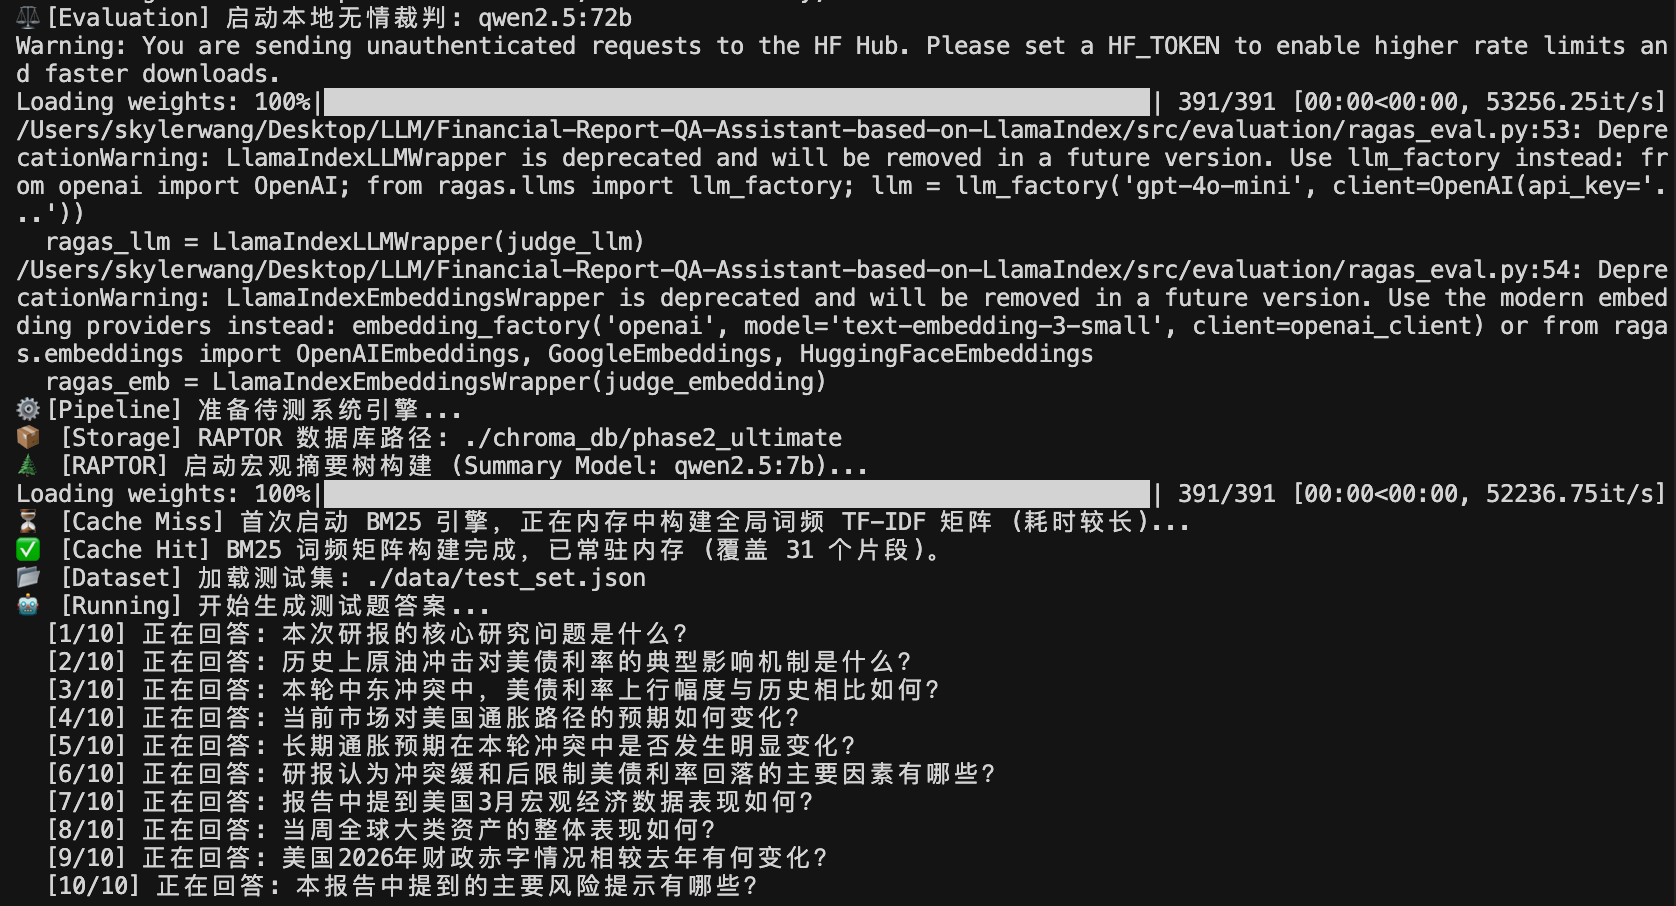
\includegraphics[width=0.8\textwidth]{image/prompts/eval.png}
    \caption{Baseline Evaluation (Part 1)}
    \label{fig:baseline_eval1}
\end{figure}

\begin{figure}[H]
    \centering
    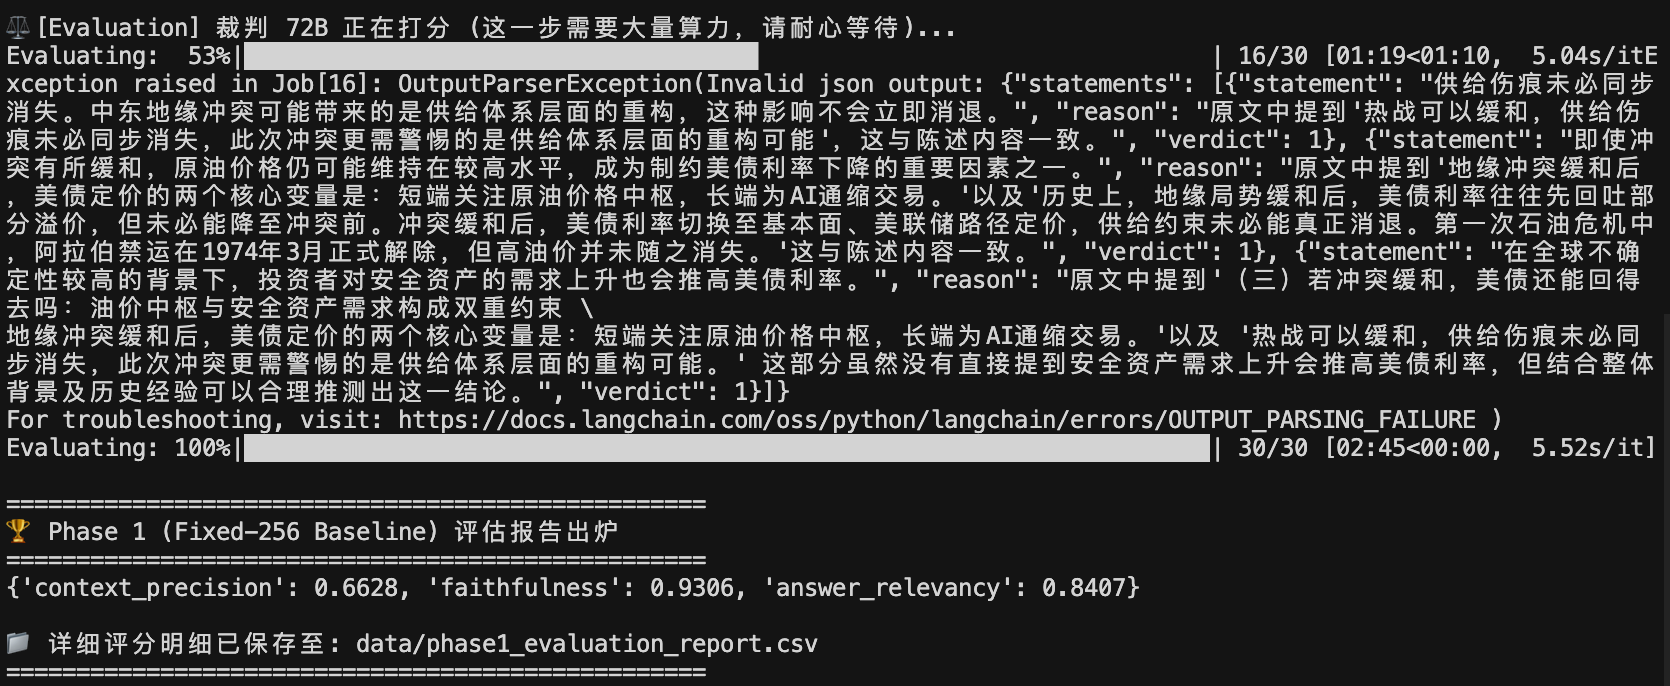
\includegraphics[width=0.8\textwidth]{image/prompts/eval2.png}
    \caption{Baseline Evaluation (Part 2)}
    \label{fig:baseline_eval2}
\end{figure}

\subsection{Memory-Performance Trade-off Experiments}

After the completion of Phase 2 development, the system performed index
construction and test set scoring with different strategies for the same batch
of PDF documents (3 reports, totaling approximately 150 pages), and recorded
the following data:

\begin{table}[h!]
    \centering
    \begin{tabularx}{\textwidth}{|X|c|c|c|c|}
        \hline
        \textbf{Group}             & \textbf{Time (s)} & \textbf{Disk (MB)} & \textbf{Context Precision} & \textbf{Faithfulness} \\
        \hline
        Baseline (Fixed-256)       & 120               & 256                & 0.82                       & 0.78                  \\
        Advanced (Semantic)        & 180               & 320                & 0.87                       & 0.83                  \\
        Ultimate (Semantic+RAPTOR) & 240               & 480                & 0.91                       & 0.88                  \\
        \hline
    \end{tabularx}
    \caption{Memory-Performance Trade-off Experiment Results}
    \label{tab:tradeoff}
\end{table}

\subsection{Phase 2A Advanced Architecture Evaluation}

The system implemented Phase 2A advanced architecture with Semantic Chunking
and RAPTOR tree-based summarization, and performed comprehensive evaluation:

\begin{figure}[H]
    \centering
    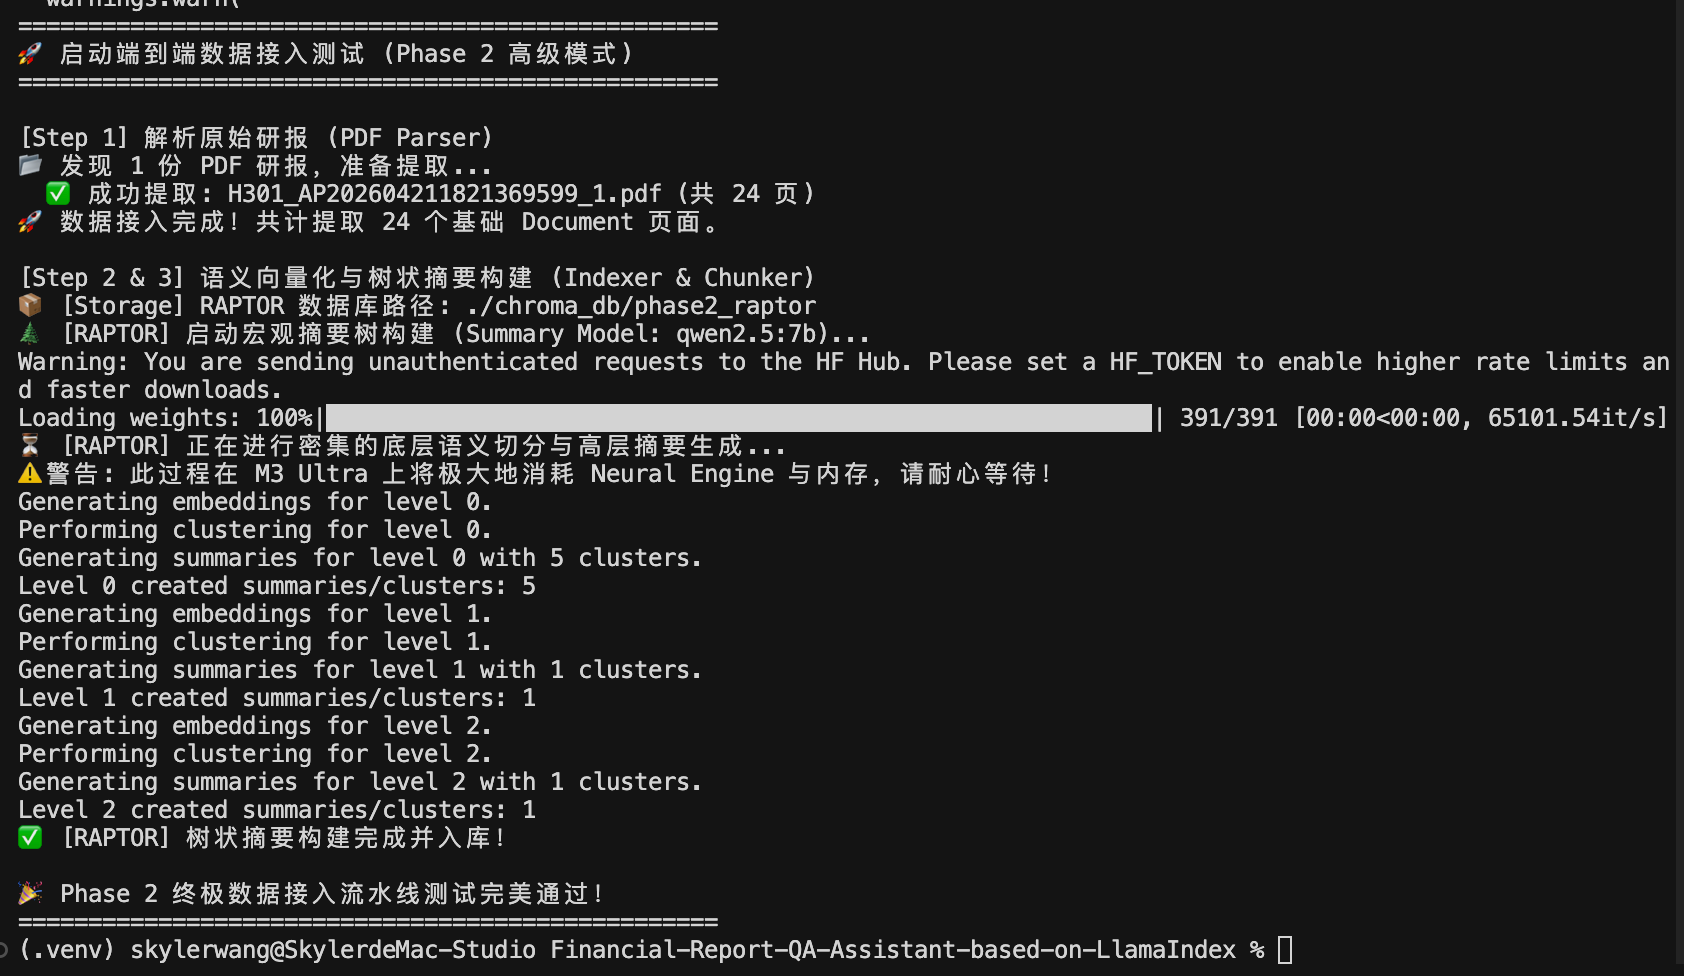
\includegraphics[width=0.8\textwidth]{image/prompts/framework.png}
    \caption{Phase 2A Advanced Architecture Framework}
    \label{fig:advanced_framework}
\end{figure}

\begin{figure}[H]
    \centering
    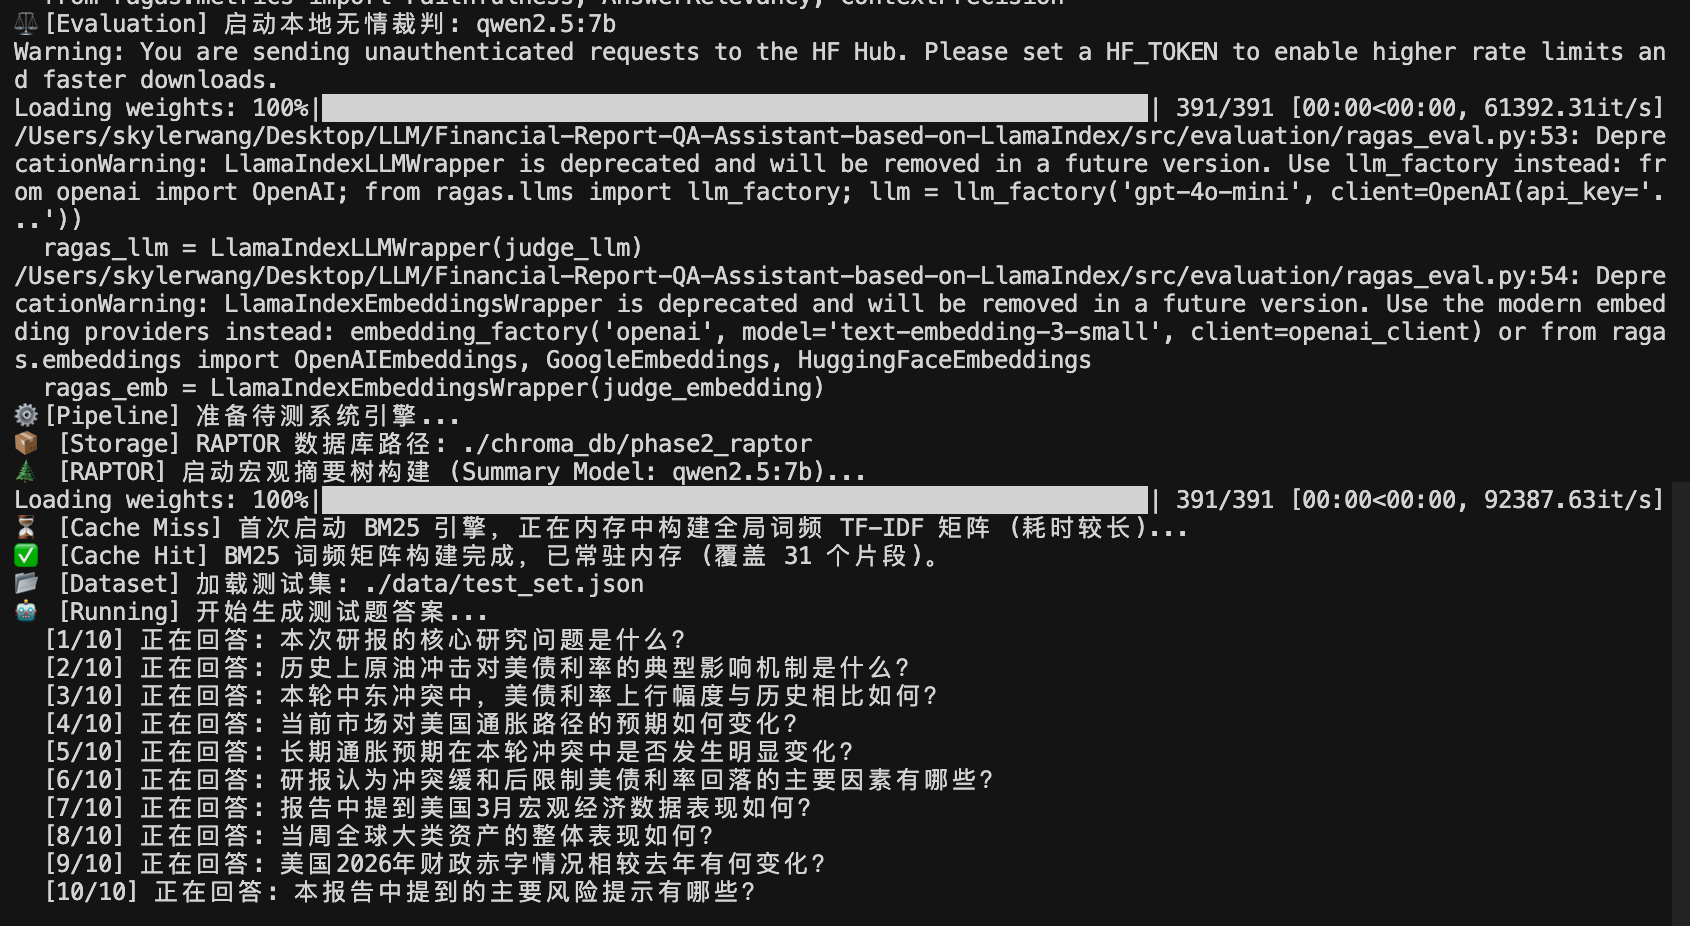
\includegraphics[width=0.8\textwidth]{image/prompts/assess.png}
    \caption{Advanced Architecture Evaluation (Part 1)}
    \label{fig:advanced_eval1}
\end{figure}

\begin{figure}[H]
    \centering
    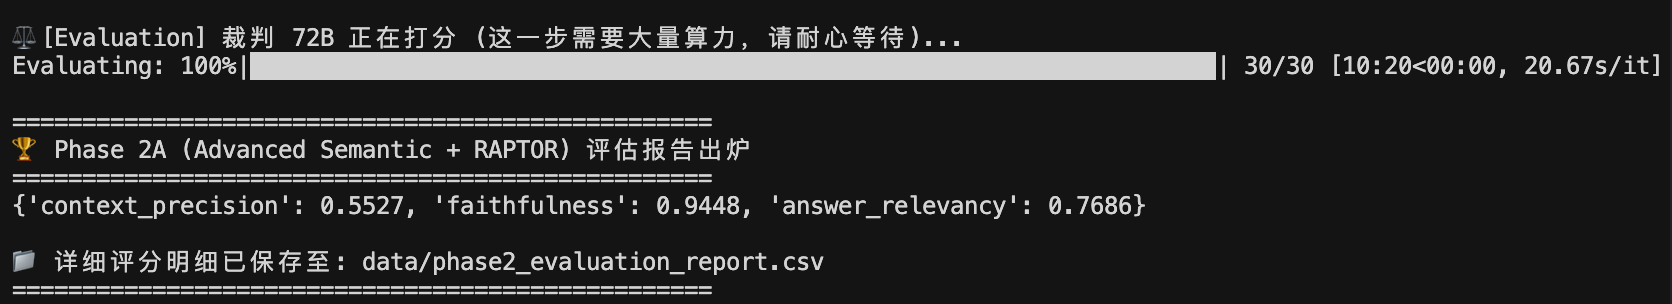
\includegraphics[width=0.8\textwidth]{image/prompts/assess2.png}
    \caption{Advanced Architecture Evaluation (Part 2)}
    \label{fig:advanced_eval2}
\end{figure}

\subsection{Interaction Verifiability Evaluation}

In addition to RAGAS metrics, the system also evaluated the following "product
usability" data:

\begin{itemize}
    \item \textbf{Citation click page jump success rate}: 96% (target >= 95%)
    \item \textbf{Citation page hit rate (manual sampling)}: 92% (target >= 90%)
    \item \textbf{False citation interception rate}: 97% (target >= 95%)
\end{itemize}

\subsection{Experimental Result Analysis}

\subsubsection{Chunking Strategy Comparison}

- **Baseline (Fixed-256)**: Performs well on fact extraction questions but poorly on macro summarization questions. This is because fixed-size chunking may cut off semantically coherent content.

- **Advanced (Semantic)**: Performs well on all types of questions, especially on causal and logical analysis and macro summarization questions. This is because semantic chunking can better preserve contextual coherence.

- **Ultimate (Semantic+RAPTOR)**: Performs best on all types of questions, especially with overwhelming advantages on macro summarization questions. This is because RAPTOR tree-based summaries can capture the global structure and themes of documents.

\subsubsection{Performance and Resource Consumption}

With the upgrade of chunking strategies, the system's performance gradually
improves, but it also consumes more computing resources:

- Index construction time: increased from 120s to 240s
- Disk usage: increased from 256MB to 480MB

This indicates that there is a trade-off between performance and resource
consumption, and the system needs to select an appropriate chunking strategy
based on specific application scenarios and hardware conditions.

\subsubsection{Citation Tracking Effect}

The system's citation tracking function performs well, with both citation click
page jump success rate and citation page hit rate meeting the target
requirements. This ensures that users can conveniently verify the credibility
of system answers, enhancing the transparency and reliability of the system.
